\begin{figure}[H]
	\centering
	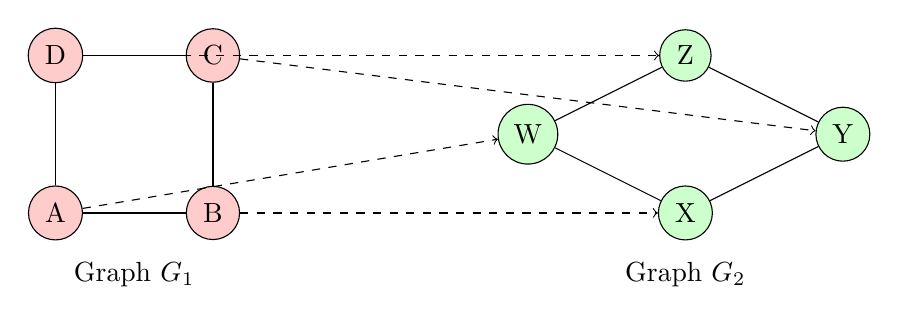
\begin{tikzpicture}
		% Graph Isomorphism - Left Graph (Square)
		\node[circle, draw, fill=red!20] (A1) at (0,0) {A};
		\node[circle, draw, fill=red!20] (B1) at (2,0) {B};
		\node[circle, draw, fill=red!20] (C1) at (2,2) {C};
		\node[circle, draw, fill=red!20] (D1) at (0,2) {D};
		\draw (A1) -- (B1);
		\draw (B1) -- (C1);
		\draw (C1) -- (D1);
		\draw (D1) -- (A1);
		\node[align=center, below] at (1, -0.5) {Graph $G_1$};
		
		% Graph Isomorphism - Right Graph (Rhombus)
		\node[circle, draw, fill=green!20] (W) at (6,1) {W};
		\node[circle, draw, fill=green!20] (X) at (8,0) {X};
		\node[circle, draw, fill=green!20] (Y) at (10,1) {Y};
		\node[circle, draw, fill=green!20] (Z) at (8,2) {Z};
		\draw (W) -- (X);
		\draw (X) -- (Y);
		\draw (Y) -- (Z);
		\draw (Z) -- (W);
		\node[align=center, below] at (8, -0.5) {Graph $G_2$};
		
		% Dashed lines indicating isomorphism
		\draw[dashed, ->] (A1) -- (W);
		\draw[dashed, ->] (B1) -- (X);
		\draw[dashed, ->] (C1) -- (Y);
		\draw[dashed, ->] (D1) -- (Z);
	\end{tikzpicture}
	\caption{Graph Isomorphism: $G_1$ (Square) and $G_2$ (Rhombus).}
	\label{fig:graph_isomorphism}
\end{figure}
